%!TEX TS-program = xelatex

\useoutertheme{infolines}

\usepackage{xetexko}
\usepackage{mathtools}
\usepackage{amsmath}
\usepackage{fontspec}
\usepackage{hyperref}
\usepackage{graphicx}
\usepackage{listings}
\usepackage{makeidx}
\usepackage{indentfirst}
\usepackage{standalone}


%\setmainfont {NanumMyeongjo}
\setsansfont {Noto Sans CJK KR}
\setmainfont {Noto Sans CJK KR}
\setmonofont[Scale=0.8]{DejaVu Sans Mono}

\lstdefinestyle{diff}{
  belowcaptionskip=1\baselineskip,
  breaklines=true,
  frame=L,
  xleftmargin=\parindent,
  showstringspaces=false,
  % Diffstart
  morecomment=[f][\color{gray}]{@@},
  % Diffincl
  morecomment=[f][\color{Green}]{+},
  % Diffrem
  morecomment=[f][\color{Red}]{-},
  basicstyle=\footnotesize\ttfamily,
}

\lstdefinestyle{customtxt}{
  belowcaptionskip=1\baselineskip,
  breaklines=true,
  frame=L,
  xleftmargin=\parindent,
  showstringspaces=false,
  basicstyle=\footnotesize\ttfamily,
}

\lstdefinestyle{customc}{
  belowcaptionskip=1\baselineskip,
  breaklines=true,
  frame=L,
  xleftmargin=\parindent,
  language=C,
  showstringspaces=false,
  basicstyle=\footnotesize\ttfamily,
  keywordstyle=\bfseries\color{green!40!black},
  commentstyle=\itshape\color{purple!40!black},
  identifierstyle=\color{blue},
  stringstyle=\color{orange},
}


\hypersetup {
  colorlinks, linkcolor=blue
}

\title {Hideroot}
\author {perillamint}


\AtBeginSection[]
{
  \begin{frame}
    \frametitle{Index}
    \tableofcontents[currentsection]
  \end{frame}
}

\begin {document}

\begin{frame}
  \titlepage
\end{frame}

% 아 일하기 진짜 싫다으아아아아

\section[Section]{루팅?}
\begin{frame}
  \frametitle{0x00. 루팅?}
  \framesubtitle{https://g.co/ABH}

  \begin{center}
    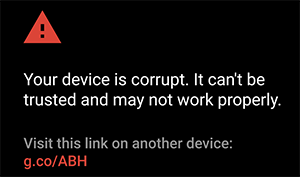
\includegraphics [width=100mm]{img/corrupted_nexus.png}
  \end{center}
\end{frame}

\begin{frame}
  \frametitle{0x00. 루팅?}
  \framesubtitle{https://g.co/ABH}

  \begin{itemize}
  \item 안드로이드 기기의 UID=0 권한을 획득하는 행위
  \item 이를 통해, 앱이 원래대로라면 가질 수 없는 권한을 획득할 수 있음
  \item 하지만 잠재적인 보안 이슈를 이유로, 많은 금융 앱들이 루트된 기기에서 동작을 거부함
  \end{itemize}
\end{frame}

\section[Section]{끝}
\begin{frame}
  \frametitle{0x0D. 끝}
  \framesubtitle{FIN}

  \begin{center}
    Q \& A
  \end{center}
\end{frame}

\begin{frame}
  \frametitle{0x0B. License}
  \framesubtitle{}
  Copyright (C)  2016 perillamint\linebreak
  Permission is granted to copy, distribute and/or modify this document
  under the terms of the GNU Free Documentation License, Version 1.3
  or any later version published by the Free Software Foundation;\linebreak
  with no Invariant Sections, no Front-Cover Texts, and no Back-Cover Texts.
  A copy of the license is included in the section entitled "GNU
  Free Documentation License".
  \linebreak
  \linebreak
  %Repository address:\linebreak
  %\url{https://github.com/perillamint/K-HomeWRT-hack}
  \linebreak
  \linebreak
  
\includegraphics [width=30mm]{img/gfdl-logo-small.png}
\end{frame}

\end {document}
